\documentclass{article}

\usepackage{float}
\usepackage[italian]{babel}
\usepackage[letterpaper,top=3cm,bottom=3cm,left=3cm,right=3cm,marginparwidth=1.75cm]{geometry}
\usepackage{amsmath}
\usepackage{graphicx}
\usepackage[colorlinks=true, allcolors=black]{hyperref}




\title{Università degli studi di Salerno
        \\Fondamenti di Intelligenza Artificiale
        \\ GCPP : Graphic Card Price Predictor}
\author{autore: Luigi Nacchia\\matricola: 0512105854}
\date{}

\begin{document}

\begin{figure}
    \centering
    
\includegraphics[width=0.95\linewidth]{logo_unisa.png}
\end{figure}

\maketitle

\newpage
\tableofcontents

\newpage
\section{Introduzione}
Negli ultimi anni, l'aumento esponenziale di mining farm e dello sviluppo modelli ML da addestrare ha portato ad un massiccio aumento della domanda di componenti hardware necessarie per tali attività, con conseguente aumento dei loro prezzi.

    \subsection{Obiettivi}
    Questo progetto di Fondamenti di Intelligenza Artificiale si propone di sviluppare un predittore del prezzo dei componenti più richiesti, le gpu.
    \\
    Gli obbiettivi principali del progetto includono:
    \begin{itemize}
        \item un'analisi dei dati delle gpu 
        \item l'identificazione delle feature più rilevanti
        \item l'implementazione di un modello di machine learning in grado di fare predizioni sul prezzo di altre gpu
    \end{itemize}
    
    \subsection{Specifica PEAS}
        \begin{itemize}
        \item Performance (misura di prestazioni): precisione e accuratezza del modello
        \item Enviroment (ambiente): i dati delle gpu 
        \item Actuators (azioni possibili): prevedere un prezzo di una gpu
        \item Sensors (percezioni possibili): acquisizione di dati di una gpu su cui fare la previsione
        \end{itemize}
    \subsection{Caratteristiche dell'ambiente}
        \begin{itemize}
        \item Parzialmente osservabile, in quanto mentre si conoscono tutte le informazioni sulle gpu nel dataset, delle altre gpu non si conosce il prezzo che deve essere predetto.
        \item Deterministico, in quanto ogni predizione è influenzata dai dati su cui il modello viene addestrato.
        \item Episodico, in quanto ogni predizione non influenza le predizioni future. 
        \item Statico, in quanto il dataset non cambia dopo una predizione
        \item Continuo, in quanto non c'è un numero massimo di possibili nuove gpu di cui predire il prezzo
        \end{itemize}
    
    \subsection{Analisi del problema}
    GCPP mira a costruire un predittore di prezzi di nuove schede sulla base di dati di altre schede il cui prezzo è noto. 
    Si tratta quindi di un problema di apprendimento supervisionato.
    Le tecnologie e strumenti che ho utilizzato per lo sviluppo del progetto sono:
        \begin{itemize}      
        \item GitHub (versioning)
        \item Overleaf (documentazione in \LaTeX)
        \item Kaggle (dataset)
        \item Python (SickitLearn, Pandas)
        \item Google Colab (notebook)
        \end{itemize}

\newpage
\section{Data Understanding}
    \subsection{Acquisizione dei dati}
    L'acquisizione dei dati è il processo di ricerca e raccolta dei dati necessari per addestrare con successo un modello di ML. 
    Con gli obiettivi chiari e definiti, sono andato alla ricerca di un dataset sulla nota piattaforma online di data-science "Kaggle".
    Il dataset che ho scelto di usare è il seguente:
    \begin{figure}[H]
    \centering
    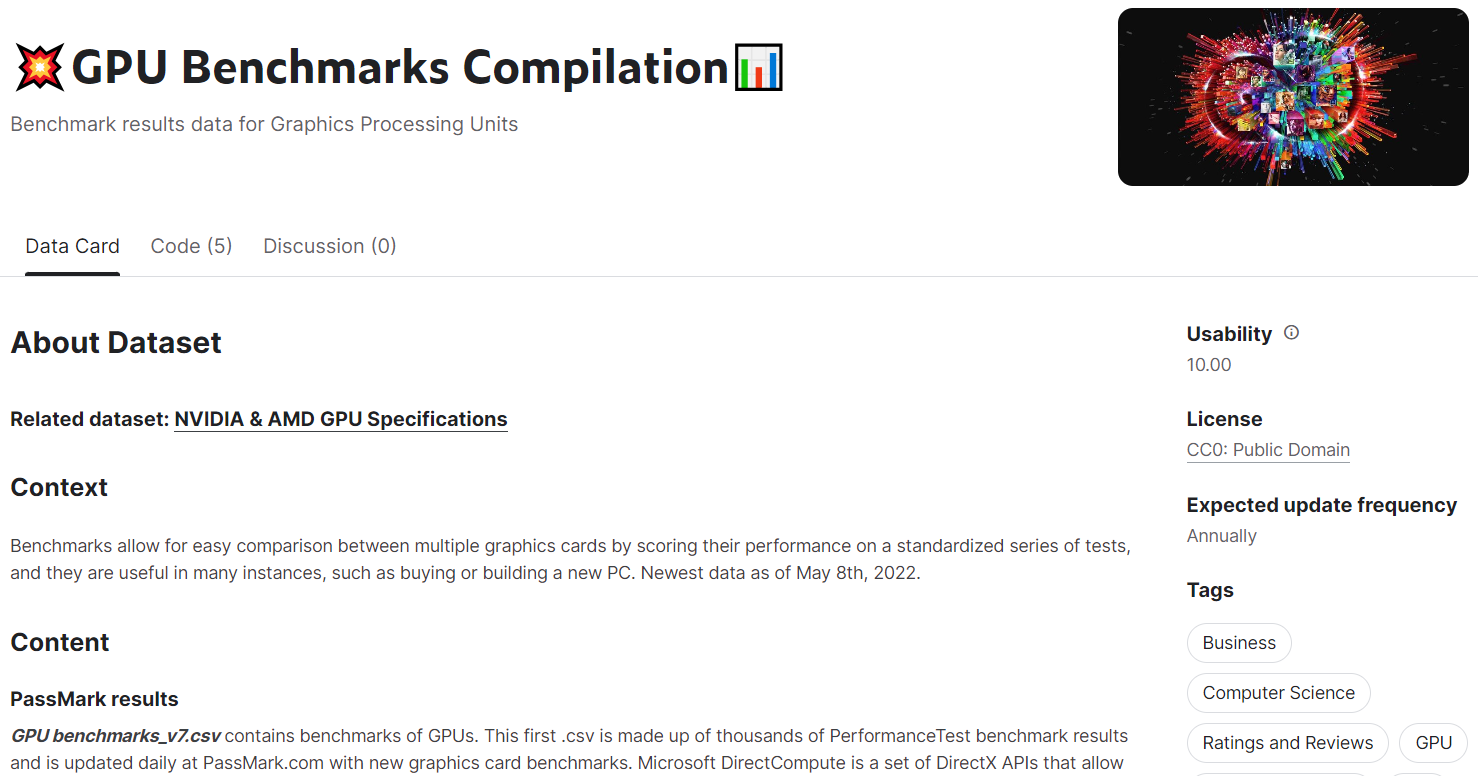
\includegraphics[width=0.95\linewidth]{kaggle_dataset.png}
    \end{figure}
    
    
    \subsection{Esplorazione dei dati}
    Il dataset "GPU Benchmark Compilation" è un insieme di dati sulle gpu.
    Nel dettaglio, per ogni gpu abbiamo dati su:
     \begin{itemize}
        \item nome univoco della scheda 
        \item misure di prestazioni (benchmark 3D/2D)
        \item prezzo in dollari
        \item consumo in Watt 
        \item anno
        \item categoria
        \item valore (prestazioni/prezzo)
        \item efficienza (prestazioni/consumi)
        \end{itemize}
    \subsection{Analisi della qualità dei dati}

\newpage
\section{Data Preparation}
    \subsection{Data Cleaning}
    \subsection{Feature Scaling}
    \subsection{Feature Selection}
    \subsection{Data Balancing}
    \subsection{Split del Dataset}

\newpage
\section{Data Modeling}
    \subsection{Scelta dell'algoritmo}
    \subsection{Addestramento}

\newpage
\section{Evaluation}

\newpage
\section{Deployment}


\end{document}
